\chapter{Probing Competition between Coherent and Dissipative Dynamics At Short Times}
\thispagestyle{empty}
\label{chap:short_time_dynamics}

In this final chapter, we will present a different approach to characterize the competition between coherent dissipative dynamics in the models that we considered in chapter~\ref{chap:MIPT_bosons} and~\ref{chap:MIPT_continuous_measurement}. The content of this chapter is the result of the author's final project, which is presented in Ref.~\cite{bintener2024}.

\section{Introduction}

In the previous two chapters, we have explored the measurement-induced phase transitions that result from the competition between coherent dynamics, which build up entanglement, and quantum correlations and measurements, which lead to the localization of information and a decrease of entanglement. The MIPTs resulting from this competition have been studied in several contexts in recent years~\cite{li2018,li2019,skinner2019} and are characterized by nonlinear functions in the density operator at long times. The time evolution of the system wavefunction follows independent measurement trajectories, where nonlinear functions, upon averaging, display qualitatively different behavior with varying measurement strength. The steady state of the models we have considered is the trivial infinite temperature state, which is reached independently of the measurement strength. Therefore, linear quantities computed from individual trajectories coincide with their expectation values in the infinite temperature state, while nonlinear functions, in general, do not. So far, we have only analyzed the steady-state properties of our models, and two interesting questions arise: Can we relax this requirement, and are we able to distinguish features of the different phases during the short-time dynamics of the system evolution? The transition only clearly is a transition in the steady state as a balance in the competition between coherent and dissipative dynamics has been reached. At short times, we expect that for very small measurement strengths, the behavior of the system is dictated by coherent dynamics. In contrast, at short times, for large measurement strengths, measurements occur so frequently that the system will tend to remain in its initial state. In between, we expect a crossover region rather than the phase transition at a critical measurement strength, as the competition between coherent and dissipative dynamics results in damped oscillations of both linear and non-linear quantities, as we will show in the following sections. Still, relaxing the requirement of only considering steady-state properties allows us to investigate linear functions of the density operator, which, as we will see, can be used to characterize not the phase transition itself but rather the competition between coherent and dissipative dynamics differently than we have seen so far. The goal remains to devise an approach that allows us to find signatures to detect the underlying many-body phenomena experimentally. We conclude this chapter with a reproducible method that allows us to characterize the different behaviors in our model using a cross-trajectory correlator, which we adapt from the protocol from Ref.~\cite{vermersch2019}. We compute the correlator by sampling directly from the infinite temperature state, and we show that although the infinite temperature state itself is featureless, we can discriminate between the area-law and intermediate regime, which is characterized by logarithmic scaling of the von Neumann entropy in the steady state. We now briefly recap the model we have encountered in chapter~\ref{chap:MIPT_bosons} and present the results for early-time dynamics of our model as well as experimental probing of the competition between coherent and dissipative dynamics.

\section{Model}

As mentioned in this chapter, we consider the model we investigated in chapter~\ref{chap:MIPT_bosons}. We consider a periodic $1$D chain that consists of hardcore bosons with nearest-neighbor hopping and first- and second-neighbor interactions, described by the Hamiltonian,
\begin{equation}
\hat{H}_\text{hop} =-J \sum\limits_{i=1}^{M} ( \hat{a}^{\dagger}_i \hat{a}_{i+1} + \textrm{h.c.}) + U_1\sum\limits_{i=1}^{M} \hat{n}_i \hat{n}_{i+1}
+ U_2\sum\limits_{i=1}^{M} \hat{n}_i \hat{n}_{i+2},
\end{equation}
with hopping parameter $J$, interaction strengths $U_1, U_2$ between first and second neighbors respectively, and the respective bosonic creation and annihilation operators $\hat{a}^\dagger_i, \hat{a}_i$. 

Furthermore, the system is subject to dephasing of the local particle numbers, with jump operators $\hat{n}_i = \hat{a}^\dagger_i \hat{a}_i$. As before, the MIPT in the steady state is not accessible through linear functions in the density operator, which is the reason why we consider a photon counting unraveling of the master equation to simulate the dynamics and access the transition. 

\section{Short-time behavior of nonlinear and linear functions}

As we have seen in chapter~\ref{chap:MIPT_bosons}, the MIPT in this model is best characterized by the von Neumann entropy in the steady state, computed in individual measurement trajectories and then averaged. In this model, the entropy at small measurement strengths scales linearly with subsystem size, exhibiting volume-law scaling. At large measurement strengths, information becomes localized due to frequent measurements, and the system is in the area-law phase, where entropy is independent of subsystem size. In the intermediate regime, the entropy grows logarithmically with subsystem size. 

As mentioned in the previous section, an interesting question that arises is how the entropy behaves at short times, which we now explore. In Fig.~\ref{fig:Chapter5_Fig1} a), d), we plot the entropy at $TJ = 1$ for the non-interacting and interacting cases, respectively. For large measurement strengths $\gamma$, the entanglement entropy exhibits area-law scaling with the subsystem size. Comparing this to the steady-state behavior in Fig.~\ref{fig:Chapter5_Fig1} c),f) and intermediate times~\ref{fig:Chapter5_Fig1} b), e), we note that the area-law behavior manifests at very short times and does not change considerably as we time-evolve. This is expected, as frequent measurements result in a Zeno-type effect, which means at the trajectory level, the system remains close to a product state with low entanglement. Therefore, there appears only a small entanglement build-up, which then remains constant. 
\begin{figure}[ht]
    \centering
    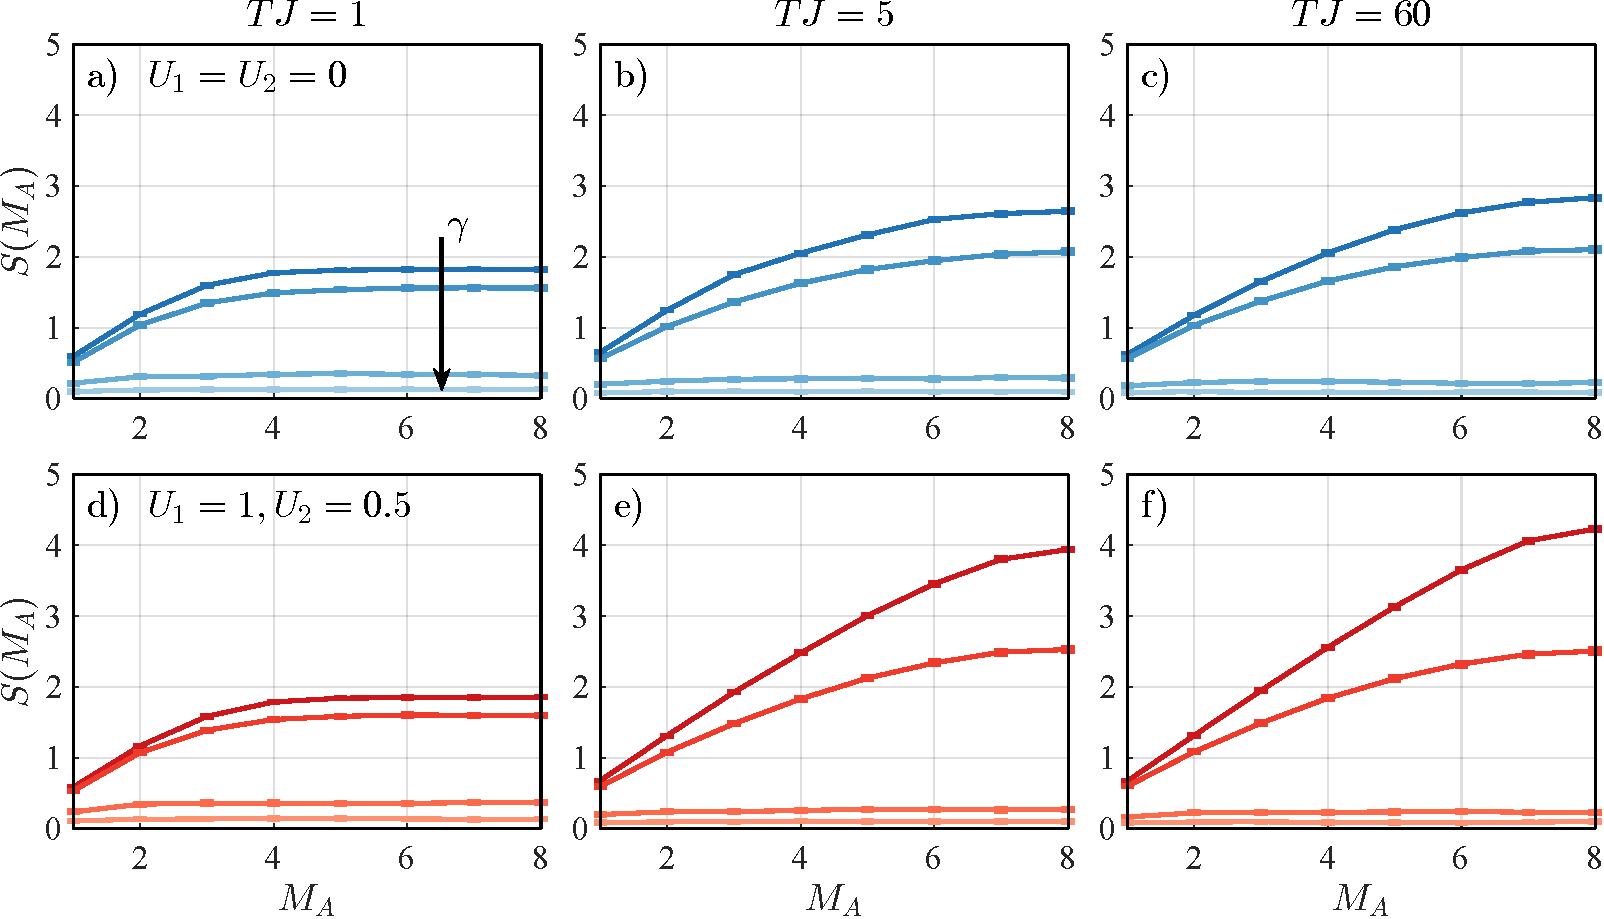
\includegraphics[width=\textwidth]{Chapters/Plots/Chapter6/Chapter5_Fig1.pdf}
    \caption{Snapshots of the von Neumann entropy at three different points in time, $TJ  = [1, 5, 60]$, as a function of subsystem size $M_A$ ($M=16$) for a)-c) the non-interacting model $U_1 = U_2 = 0$, and d)-f) the interacting model with $U_1 = 1, U_2 = 0.5$. We display the entropies for dissipation strengths, $\gamma \in [0.1,0.5,5,10]$, increasing in the direction of the arrow in a). For each snapshot, we time-evolve until $TJ = [1, 5, 60]$, and compute trajectory averages using $N_t = 300$ trajectories.}
    \label{fig:Chapter5_Fig1}
\end{figure}
On the other hand, however, for small measurement rates and at short times, for $TJ = 1$, we see for both the interacting and non-interacting cases in Fig.~\ref{fig:Chapter5_Fig1}a),d) that the entanglement grows with subsystem size to around a subsystem size around $M_A \sim 4$. As only a little time has passed, correlations have not spread further through the system, and hence, at larger subsystem sizes, the entanglement entropy remains constant. At long times for this system size, $TJ = 5$, we now see the entropy behavior in Fig.~\ref{fig:Chapter5_Fig1} b),e) coincides with the steady-state behavior. However, the important conclusion we draw from this analysis is that the qualitative behavior already manifests in the entropy at short times. The quantitative differences arise due to coherent oscillations of the entropy at short times and small measurement strengths. Still, once correlations have been able to travel through the whole system, the qualitative entropy behavior becomes apparent, and we can distinguish the different phases effectively by studying the scaling with time and subsystem size. Note that since we only consider specific snapshots in time, the quantitative entropy behavior changes at intermediate times as a function of the choice of time, which is also a reason why we do not expect to detect the transition itself but rather a crossover region, where features of the transition are already present.

As we have seen, it is possible to clearly distinguish the two regimes, even at early times, where coherent dynamics are still competing with the measurements. Being able to focus on early time dynamics also gives us the advantage of analyzing linear quantities. Starting from a state with all particles initially in odd sites, coherent time evolution allows the particles to hop to neighboring sites and occupy even sites. The coherent time evolution is interrupted by random projective measurements. For small measurement strengths, the unitary time evolution leads to tunneling of the particle to neighboring sites, and projective measurements only rarely occur. In the large measurement regime, measurements occur frequently and project the particles often in odd sites, as they are not able to tunnel to neighboring sites. We further comment on this later in the chapter. To characterize the competition between the coherent dynamics and local projective measurements, we consider the imbalance, defined as the difference between the sum of local densities in event and odd sites,  
\begin{equation}
    \label{eq:imbalance}
    I = (N_e - N_o)/N = \frac{\sum_i (-1)^i \expectation{\hat{n}_i}}{\sum_i  \expectation{\hat{n}_i}},
\end{equation}
where $N_e, N_o$ are the total particle numbers in even and odd sites, respectively, and $N = N_e+N_o$ is the total particle number. For our analysis, we consider an initially imbalanced product state, with all particles in odd sites, and explore how the imbalance relaxes in the presence of measurements. With all particles initially in odd sites, $N_e(t=0) = 0$, and $N_o(t=0) = N$, we have $I(t=0) = -1$. In our model for non-zero measurement rates, at long times, the system loses all information about the initial state, and the average particle number for site $i$ is $\expectation{\hat{n}_i} = 1/2$, hence $I(t\to \infty) = 0$ for all $\gamma \neq 0$. We will now explore the early-time dynamics of the population imbalance and analyze how it relaxes from $-1$ to $0$. 

\begin{figure}[ht]
    \centering
    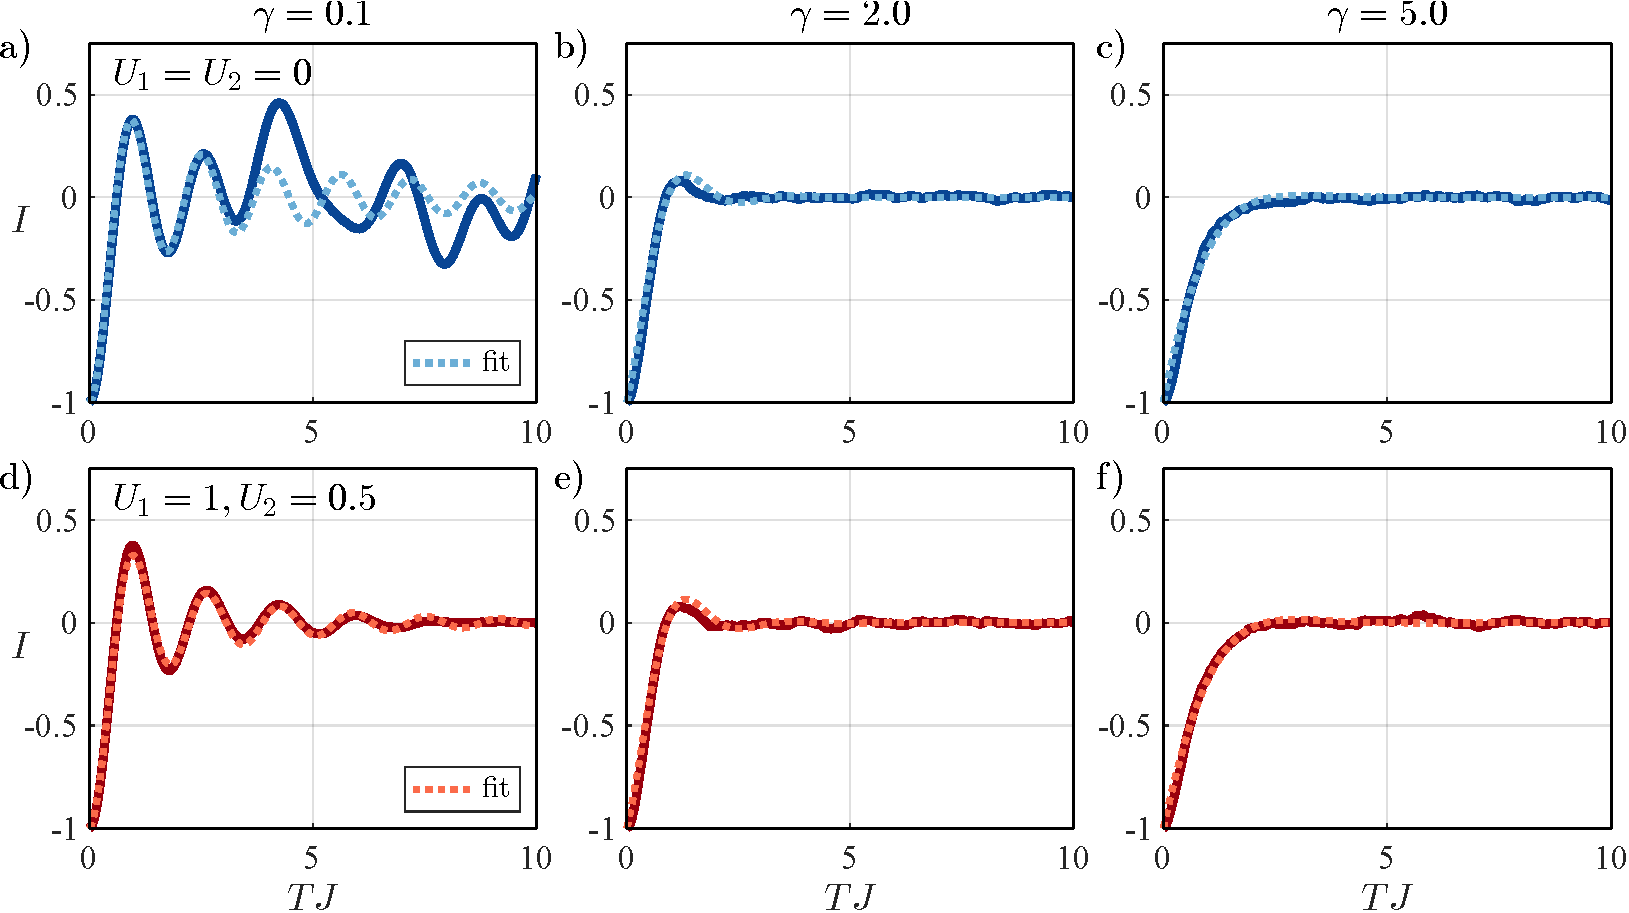
\includegraphics[width=\textwidth]{Chapters/Plots/Chapter6/Chapter5_Fig2.pdf}
    \caption{The population imbalance for a)-c) the non-interacting model $U_1 = U_2 = 0$, and d)-f) the interacting model with $U_1 = 1, U_2 = 0.5$. We display three measurement strengths: a),d) $\gamma=0.1$, b),e) $\gamma=2$, and c),f) $\gamma=5$. For each curve, we also compute a fit of the form $f(t) = J_0(at) e^{-\Gamma t}$, where $J_0$ is the zeroth-order Bessel function of the first kind and fitting parameters $a, \Gamma$. We compute trajectory averages using $N_t = 300$ trajectories.}
    \label{fig:Chapter5_Fig2}
\end{figure}

In Fig.~\ref{fig:Chapter5_Fig2} a),d), we consider the evolution of the imbalance for the measurement strength $\gamma = 0.1$ for the non-interacting and interacting models. In the non-interacting model, finite-size effects are relatively prominent; however, in the interacting model, we can observe dampened coherent oscillations resulting from the competition between the coherent and dissipative dynamics. In the strong measurement regime, depicted in Fig.~\ref{fig:Chapter5_Fig2} c),f), for $\gamma = 5$, the oscillations are fully suppressed as the measurements dominate the dynamics in the system. From our analysis in Chap.\ref{chap:MIPT_bosons} we expect a transition from logarithmic to area-law scaling of the entropy around $\gamma = 2$ and we, therefore, display the imbalance in Fig.~\ref{fig:Chapter5_Fig2} b),e) for this measurement strength. There are no clear visible oscillations for this measurement strength; however, we observe a small increase in the value before the imbalance remains constant around $0$. This analysis clearly shows the competition between the measurements and coherent time evolution, with indications of a transition in the qualitative behavior at around $\gamma = 2$. 

To better understand and analyze the behavior of the imbalance, we also include a fit to the data in Fig.~\ref{fig:Chapter5_Fig2}. In the absence of measurements, the population imbalance in this model follows a zeroth-order Bessel function of the first kind \cite{barmettler2009}. As the coherent oscillations are increasingly stronger damped with growing measurement rate, we characterize the nature of the damping by fitting an exponentially decaying Bessel function to our data of the form, 
\begin{equation}
    f(t) = J_0(at) e^{-\Gamma t},
\end{equation}
where $J_0$ is the zeroth-order Bessel function of the first kind with fitting parameters $a, \Gamma$. In Fig.~\ref{fig:Chapter5_Fig2}, we generally observe good agreement between the fit and the simulated data. In the non-interacting model for small measurement rates, we observe some significant deviations from the fit, which are the result of finite-size effects in the simulation. These deviations, however, are only present for $\gamma < 0.5$ in the non-interacting model, and we otherwise have good agreement with our data and a coefficient of determination $R^2 \approx 1$. 

\begin{figure}[ht]
    \centering
    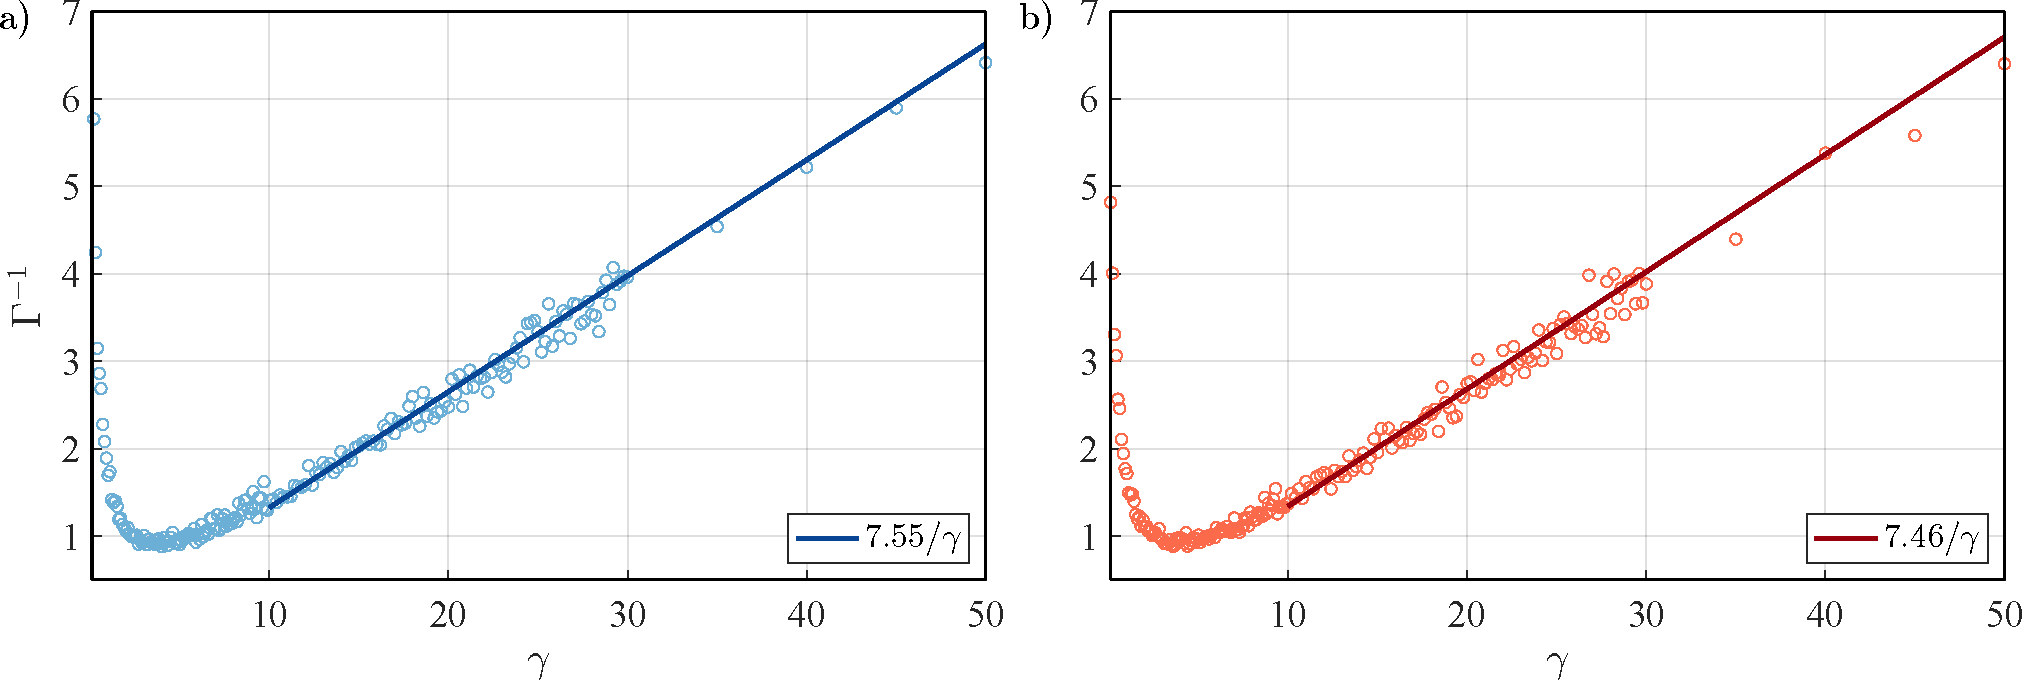
\includegraphics[width=\textwidth]{Chapters/Plots/Chapter6/Chapter5_Fig3.pdf}
    \caption{The fitted damping parameter $\Gamma$ as a function of the measurement strength $\gamma \in [0.1,50]$ for a) the non-interacting model $U_1 = U_2 = 0$, and b) the interacting model with $U_1 = 1, U_2 = 0.5$. The solid lines are fitting functions of the form $f(\gamma) = a/\gamma$ as indicated in the respective legends.}
    \label{fig:Chapter5_Fig3}
\end{figure}

In Fig.~\ref{fig:Chapter5_Fig3}, we analyze the behavior of the damping rate $\Gamma$, and we observe an initial increase of the damping rate $\Gamma$ with increasing measurement strength, indicated by the downward trend of $1/\Gamma$. As the measurements occur more frequently, the coherent oscillations become increasingly suppressed, matching our expectations from the analysis in Fig.~\ref{fig:Chapter5_Fig2}. Once we reach the strong measurement regime, the quantum Zeno effect takes over as particles remain trapped in the initial state for long times and only rarely hop to neighboring sites. Due to this effect, the origin of the suppression of coherent oscillation changes as now the damping rate $\Gamma$ decreases with the measurement strength $\gamma$. 

To better understand the behavior of the damping rate $\Gamma$, let us consider a simple system where only one particle is present in the system at site $j$. The average time between measurements is $1/\gamma$, and after this time, the state has evolved according to 
\begin{equation}
    \ket{\psi(t = 1/\gamma)} = e^{-i H / \gamma} \ket{\psi(t=0)}.
\end{equation}
When $\gamma \gg J$, the system will not have had a lot of time to evolve, and after time $1/\gamma$, the particle will be at site $j$ with amplitude $\sim 1$ or at one of its neighboring sites with amplitude $i J/\gamma$. Then, the measurement projects the particle onto its initial site with probability $\sim 1$ or onto one of its neighboring sites with probability $J^2/\gamma^2$. Therefore, we expect that this process occurs at a rate $J^2 / \gamma$ in the large measurement regime. We confirm that this expectation matches the data as we can observe the linear scaling of the inverse of the damping rate Gamma in Fig.~\ref{fig:Chapter5_Fig3} for large measurement strengths, $\gamma \geq 10$. The scatter points correspond to the simulated data points of the damping parameter $\Gamma$. We then consider a fitting function of the form $f(\gamma) = a/\gamma$, which we fit in the interval $\gamma \in [10, 30]$. We plot the inverse of the fitting function, $f(\gamma)^{-1}$ as a solid line, extending it to the range $[10, 50]$ and see that data points $\gamma > 30$ also follow the trend of the fitted solid line, indicating we have a good fit to the simulated data. 

This analysis suggests that although we are considering a linear function at short times, we can differentiate the area-law regime from the critical regime. Moreover, this analysis seems to fail to find evidence of a volume-law phase in the interacting model for small measurement strengths, which is consistent with the analysis from our previous chapters, where the detection of a volume-law phase has proven to be much more difficult than the transition from the intermediate to the area-law regime. 

\section{Experimental probing of the competition between coherent and dissipative dynamics}

So far, we have seen that non-linear quantities, such as the von Neumann entropy, exhibit signatures in the steady state that allow us to distinguish between the area-law and logarithmic regimes in our model as a function of the measurement strength. Furthermore, experimental detection of the transition using non-linear functions in the density operator is impractical as measurement outcomes are often not reproducible, and techniques for measuring the entropy cannot be used. In the previous section, we have shown that the population imbalance at early times may also be used to detect some features of the transition. In the model we are considering, the population imbalance oscillates due to the competition between coherent time evolution and projective measurements that localize system information. With increasing measurement rates, the oscillations become increasingly suppressed. This allows us to highlight a regime where oscillations become fully suppressed, and the projective measurements dominate the dynamics of the system. Although we cannot study the transition itself using linear quantities at short times, we are able to detect some features that we used to characterize the transition in Chap.~\ref{chap:MIPT_bosons}. 

With this in mind, we will consider a protocol that allows us to probe non-linear correlations at short times in a way that avoids having to access trajectories multiple times. The protocol is based on ideas proposed in Refs.~\cite{elben2018,vermersch2018, vermersch2019}, which allows us to sample the infinite temperature state and extract non-linear information in an experimentally feasible way. We will show that with this protocol, we are able to witness features of the transition by considering the cross-correlations between different measurement trajectories at short times, using random initial states.

\subsection{Protocol}

We begin by preparing an initial product state, $\ket{\psi_0}$, to which we apply local random rotations, 
\begin{equation}
\label{eq:Ru}
    \ket{\psi_0}_u = R_1 \otimes R_2 \otimes ... \otimes R_M \ket{\psi_0} = R_u \ket{\psi_0},
\end{equation}
where $M$ are the lattice sites, and $R_i$ are local random rotations drawn from the circular unitary ensemble (CUE). It can be shown that by averaging over random rotations, we approach the infinite temperature state with increasing precision as we increase the number of random rotations $N_u$ over which we average,
\begin{equation}
    E\big[\ket{\psi_0}\bra{\psi_0}_u\big] = \mathcal{I}/2^M,
\end{equation}
where $E[\cdot]$ denotes the average over many random rotations. This allows us to reliably sample the infinite temperature state and investigate the early-time dynamics using randomly rotated states. 

 In Ref.~\cite{vermersch2019}, the authors develop a protocol to measure out-of-time-ordered correlation (OTOC) functions. OTOCs have been found to be particularly interesting for studying quantum chaos \cite{cotler2018} and quantifying how information travels through many-body quantum systems \cite{hosur2016, chen2016,fan2017,nahum2018a, vonkeyserlingk2018a}. The experimental scheme they propose relies on measuring correlations between local operators, and they prove that it corresponds to the OTOC. In order to measure the cross-correlations between measurement trajectories in our model, we adapt the scheme proposed in Ref.~\cite{vermersch2019}, and we will show that we can use it to highlight features of the transition. 
 
 In particular, the quantity we propose to investigate is the cross-trajectory two-point correlator between local densities,
\begin{equation}
\label{eq:otoc_ru}
    O^{(\hat{n}_i,\hat{n}_j)}(t)= \frac{ E\big[\expectation{\hat{n}_j(t)} \expectation{\hat{n}_i(0) \hat{n}_j(t) \hat{n}_i(0)} \big] }{ E\big[\expectation{\hat{n}_j(t)}^2\big]}.
\end{equation}
where $\hat{n}_i$ is the local number operator acting at site $i$. We now outline the steps in Protocol~\ref{alg:protocol1} required to measure the correlator defined in Eq.~\ref{eq:otoc_ru}.

\begin{figure}[ht]
\begin{algorithm}[H]
\floatname{algorithm}{Protocol}
\caption{Measurement of $O^{(\hat{n}_i,\hat{n}_j)}$}
\label{alg:protocol1}
\renewcommand{\thealgorithm}{}
\begin{algorithmic}[1]
\State Prepare a product initial state $\ket{\psi_0}$ and apply the local random rotation to obtain $\ket{\psi_0}_u = R_u \ket{\psi_0}$, following Eq.~\ref{eq:Ru}. 
\State Apply the operator $\hat{n}_i$ to the randomly rotated state $\ket{\psi_0}_u$. 
\State Time-evolve it using standard quantum trajectory methods to the chosen time $T$ and measure the operator $\hat{n}_j$.
\State Repeat steps 1. and 3. with the same random rotation $R_u$ and measure $\hat{n}_j$ without first applying the local operator in step 2. 
\State Repeat steps 1. - 4. for $N_u$ random rotations and estimate $O^{(\hat{n}_i,\hat{n}_j)}$ using Eq.~\ref{eq:otoc_ru}. 
\end{algorithmic}
\end{algorithm}
\end{figure}

With this protocol, we sample the states from the infinite temperature state, and we can measure $O^{(\hat{n}_i,\hat{n}_j)}$ to investigate the short-time behavior of the system. Another critical factor is that we need to verify that our protocol also works in an experimental setting. To simulate an experimentally detected correlator $\tilde{O}^{(\hat{n}_i,\hat{n}_j)}$, we follow the same steps as in Protocol~\ref{alg:protocol1}, and instead of using the quantum mechanical expectation values, we simulate the experimental expectation values by randomly drawing a $1$ with probability $\expectation{\hat{n}_j(t)}$ and with the default being a $0$. In this way, we can test whether or not our proposed correlator is able to withstand additional noise. 

\subsection{Analysis of the correlator}

Now that we have discussed the protocol, we will look at the short-time dynamics of the correlator in our system. In Fig.~\ref{fig:Chapter5_Fig4}, we plot the correlator $O^{(\hat{n}_i,\hat{n}_j)}(t)$ as a function of time and space, where we chose $\hat{n}_i = \hat{n}_{M/2}$ as local operator to apply at $t=0$. As in our previous analysis, there is almost no qualitative difference between the non-interacting and interacting models, but we observe different behavior based on the measurement strength.

\begin{figure}[ht]
    \centering
    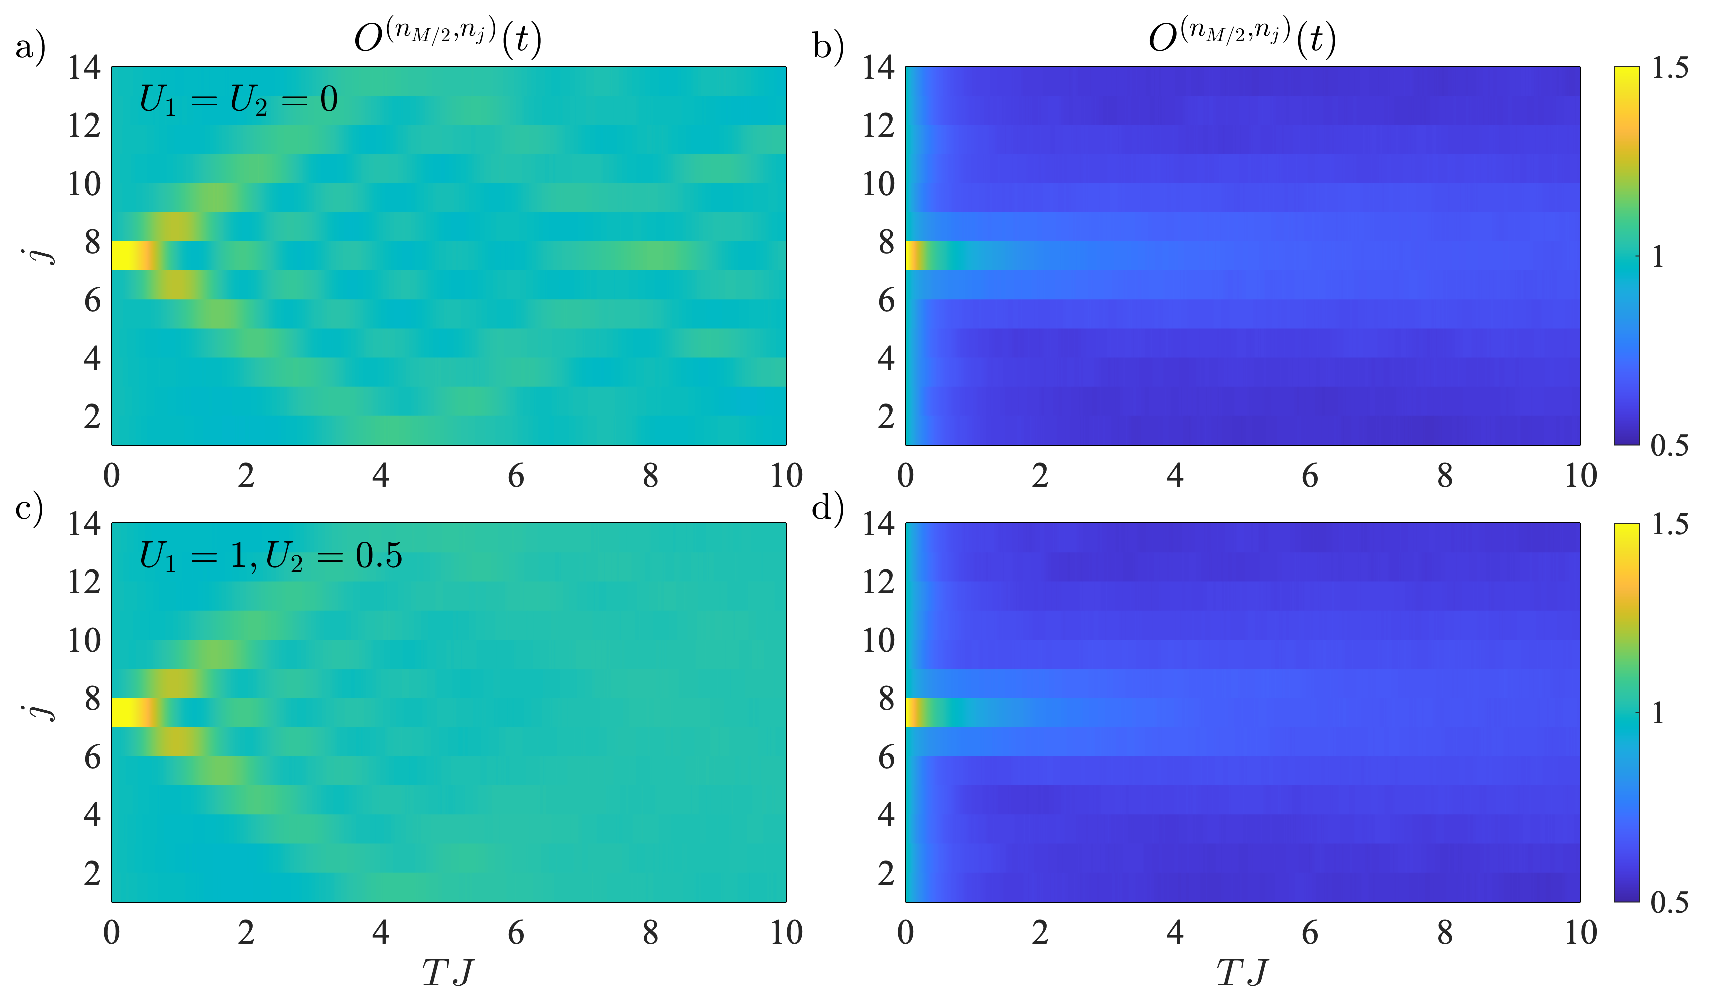
\includegraphics[width=\textwidth]{Chapters/Plots/Chapter6/Chapter5_Fig4.pdf}
    \caption{We plot the correlator $O^{(\hat{n}_{M/2},\hat{n}_j)}(t)$ a), c) for the measurement rates $\gamma = 0.1$ and b), d) $\gamma = 5$ and compare the non-interacting and interacting cases in a), b) $U_1 = U_2 = 0$ and c), d) $U_1 = 1, U_2 = 0.5$. The system consists of $M=14$ sites and time evolve over a range $TJ \in [0, 10]$ using a numerical time step $dt = 10^{-3}$ and average over $N_u = 10^4$ trajectories.}
    \label{fig:Chapter5_Fig4}
\end{figure}

In Fig.~\ref{fig:Chapter5_Fig4}, at $t=0$, the two terms in the numerator differ only at the central site where the operator was applied, highlighting the localized particle. For a small measurement rate $\gamma = 0.1$, we can observe ballistic operator spreading and coherent oscillations traveling through the system. In the interacting model, we additionally see that the oscillations stop after the operator spreading has reached the boundary of the system and the correlator reaches approximately steady behavior around $1$. For a large measurement rate $\gamma = 5$, there appear to be no qualitative differences, and the spreading appears reminiscent of a single particle diffusing in an empty lattice under continuous monitoring. Furthermore, the correlations decay to a value around $0.5$, and the coherent oscillations we saw for the small measurement rate case are fully suppressed by the dissipative dynamics. 

\begin{figure}[ht]
    \centering
    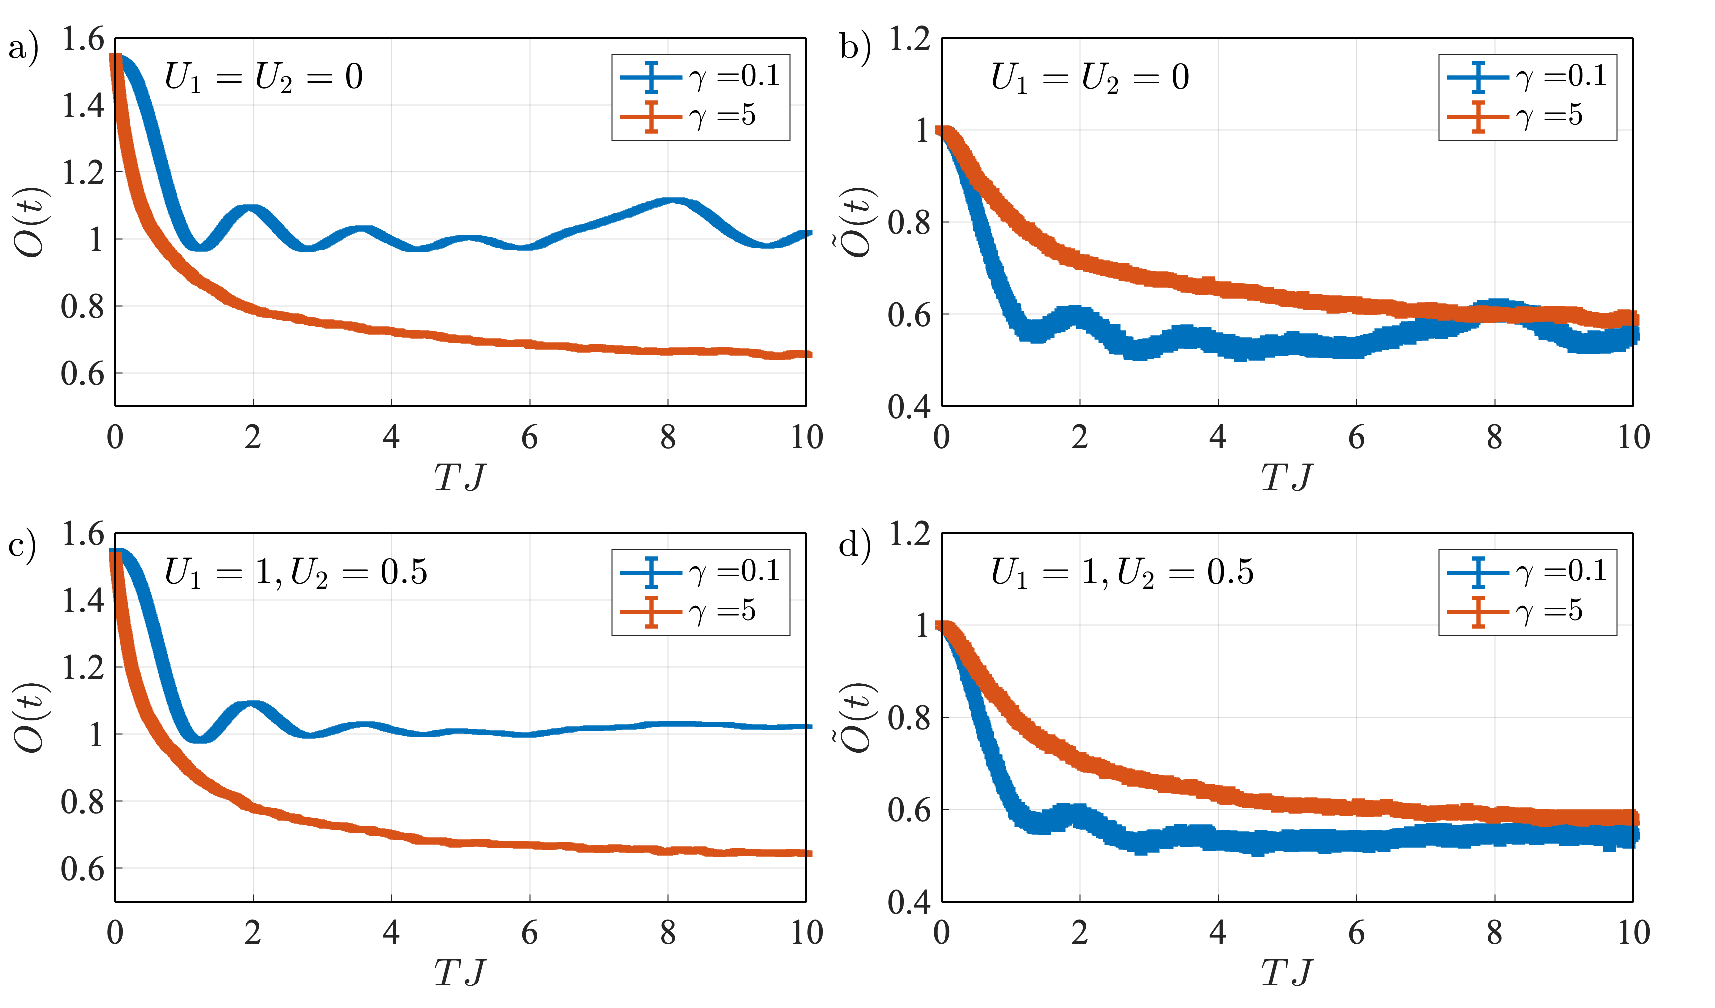
\includegraphics[width=\textwidth]{Chapters/Plots/Chapter6/Chapter5_Fig5.pdf}
    \caption{We plot a), c) the correlators $O^{(\hat{n}_{M/2},\hat{n}_{M/2})}(t) \equiv O(t)$ and b), d) $\tilde{O}^{(\hat{n}_{M/2},\hat{n}_{M/2})(t)} \equiv \tilde{O}(t)$ with $\hat{n}_i = \hat{n}_j = \hat{n}_{M/2}$ as a function of time for varying measurement rates. We compare a), b) the non-interacting, and c), d) the interacting cases. We consider a system of $M=14$ sites and time evolve over a range $t \in [0, 10]$ using a numerical time step $dt = 10^{-3}$ and $N_u = 10^4$ trajectories.}
    \label{fig:Chapter5_Fig5}
\end{figure}

We now more closely analyze the behavior of the correlator at the central site, where we compare $O^{(\hat{n}_i,\hat{n}_j)}$ and $\tilde{O}^{(\hat{n}_i,\hat{n}_j)}$, choosing operators $\hat{n}_i = \hat{n}_j = \hat{n}_{M/2}$. In Fig.~\ref{fig:Chapter5_Fig5}a), c) we plot the correlator in the small and large measurement regimes. The initial behavior for small measurement rates is similar to what we observed for the imbalance; there is an initial drop, and then oscillations appear as we evolve the system in time. In the non-interacting model, in Fig.~\ref{fig:Chapter5_Fig4}~a), we witnessed that once correlations reach the boundary, they travel back towards the center and interact. We also observe this in Fig.~\ref{fig:Chapter5_Fig4}~a), where correlations are damped but around $TJ=5$ increase again and oscillate. In contrast, in the interacting model, this effect is much less prominent, and we observe that around $TJ=5$, the correlator approaches a value $\sim 1$. In the strong measurement regime, however, oscillations due to coherent dynamics are completely washed out, allowing us to distinguish between these two regimes clearly. When we consider the correlator computed from simulated experimental expectation values, in Fig.~\ref{fig:Chapter5_Fig5}b), d), the same qualitative behavior in the two regimes appears. The oscillations in the small measurement regime are weaker due to the additional noise; however, we can still clearly distinguish the dominant coherent behavior in the small measurement regime from the strongly damped behavior in the large measurement regime. 

This analysis shows that we are able to distinguish between the two measurement regimes in both the interacting and non-interacting case, characterized by clear oscillations in the small measurement regime, which are fully damped in the large measurement regime. Since we chose $\hat{n}_i = \hat{n}_j = \hat{n}_{M/2}$, the measurement projects the particle in site $M/2$ at time $t=0$, which means we have, $\expectation{\hat{n}_i(0) \hat{n}_j(0) \hat{n}_i(0)} = 1$ and we obtain,
\begin{equation}
\label{eq:otoc_0}
    O(t=0) = \frac{ E\big[\expectation{\hat{n}_j(0)}\big] }{ E\big[\expectation{\hat{n}_j(0)}^2\big]}.    
\end{equation}
The random rotation of the state leads to a uniform distribution of the expectation values $\expectation{\hat{n}_j(0)} \sim U(0,1)$, with mean $E\big[\expectation{\hat{n}_j(0)}\big] = 1/2$. Given this, we can also find the mean of the distribution of the square $E\big[\expectation{\hat{n}_j(0)}^2\big]$. For simplicity, let us define $\expectation{\hat{n}_j(0)} \equiv N$. First, we need to find the cumulative probability function, 
\begin{equation}
    F_{N^2}(x) = P(N^2 \leq x) = P(0 \leq N \leq \sqrt{x}) = \int_0^{\sqrt{x}} dx = \sqrt{x},
\end{equation}
for $x\in[0,1]$ and using the fact that $N \sim U(0,1)$, where $U(0,1)$ is a uniform distribution on the interval $(0,1)$. To find the cumulative density function $f_{N^2}(x)$, we simply need to compute the derivative of $F_N^2$, 
\begin{equation}
    f_{N^2}(x) = \frac{d}{dx} F_{N^2}(x) = \frac{d}{dx} \sqrt{x} = \frac{1}{2\sqrt{x}},
\end{equation}
for $x\in[0,1]$. Finally, we can compute the mean of the distribution of the squared expectation values,
\begin{equation}
    E\big[\expectation{\hat{n}_j(0)}^2\big] = \int_0^1 x~f_{N^2}(x)~dx = \frac{1}{3}. 
\end{equation}

Substituting both values into Eq.~\ref{eq:otoc_0}, we obtain,
\begin{equation}
    O(t=0) = \frac{1/2}{1/3} = \frac{3}{2},    
\end{equation}
which matches the numerical data in Fig.~\ref{fig:Chapter5_Fig5}.

To compute the expected value at $t=0$ for the experimentally simulated correlator, Eq.~\ref{eq:otoc_0} still holds, however, we need to replace $\expectation{\hat{n}_j}(0)$ with $\expectation{\tilde{n}_j}(0)$, where $\tilde{\cdot}$ denotes that we replace the quantum mechanical expectation value with a $1$ with probability $\expectation{\hat{n}_j}(0)$ and a $0$ otherwise. Given a large enough sample size, when we compute the mean, it remains $1/2$. Since all values are either $0$ or $1$, however, this implies that the distribution of the squares remains unchanged and the mean of $\expectation{\tilde{n}_j}(0) = 1/2$.

Hence, we obtain, 
\begin{equation}
    \tilde{O}(t=0) = \frac{1/2}{1/2} = 1, 
\end{equation}
which also matches our numerical data. Interestingly, the dynamics of the correlator $O(t)$ are still captured by the simulated correlator $\tilde{O}(t)$, giving us an experimentally feasible protocol to show the behavioral difference of this quantity in the two regimes. 

This protocol, however, does have some drawbacks; namely, firstly, for the numerical simulation, we need a very small numerical time step, making it slower and, secondly, a large number of trajectories is needed to reduce the statistical noise enough to distinguish the signals in the two regimes. Since we are sampling the infinite temperature state, we need approximately $N_u \propto 2^M$ trajectories in order to get an accurate experimental signal. Due to these limitations, it becomes difficult to simulate larger systems as well as detect these quantities experimentally when the number of trajectories grows exponentially with the system size.

\section{Conclusion}

In this chapter, we further analyzed the competition between coherent and dissipative dynamics in a bosonic system, with and without interactions, by probing the small and large measurement regimes using linear and nonlinear functions in the density operator at short times. In chapter~\ref{chap:MIPT_bosons}, we showed the MIPT can be visualized using non-linear quantities, such as the von Neumann entropy at long times, and we can clearly distinguish between volume-law and area-law entanglement phases. The experimental detection of the MIPT proved to be a difficult obstacle, as measuring non-linear quantities requires accessing individual trajectories multiple times. Quantities that are linear in the density operator are not able to distinguish between the phases as the steady state is the featureless infinite temperature state. The main idea of this chapter was to relax these constraints of needing non-linear quantities at long times and instead analyze linear quantities at short times to find out whether or not this still allows us to distinguish features associated with the two phases, even if we cannot access the transition itself at short times. We first considered the von Neumann entropy to investigate whether the phase transition would still be present at short times, and we saw that for large measurement strengths, the entropy barely increases and already at very short times ($TJ \sim 1$) has reached its steady-state value. For small measurement strengths, however, the entropy still changes considerably at short times. However, its qualitative behavior is already clearly visible in small subsets of the whole system. This is due to the fact that correlations have not yet traveled through the system, but as the measurements occur infrequently in this regime, coherent dynamics dominate the behavior of the system. We next analyzed what happens to the population imbalance, which is defined as the difference between the population at odd and even sites normalized to the total particle number. This quantity is linear in the density operator and will approach $0$ as the local densities approach $1/2$ at long times for any non-zero measurement strength. In a system not subjected to measurements, the imbalance is described by a zeroth-order Bessel function. By introducing measurements, we saw that the coherent oscillations are increasingly suppressed with increasing measurement strengths. By fitting an exponentially decaying Bessel function, we were able to show that first, the strength of the damping increases with increasing measurement strength. After some point, due to the quantum Zeno effect, the damping rate decreases again, but oscillations continue to be increasingly suppressed as the particles remain trapped in the initial state for long times. It is interesting that this change occurs in the same regime where we expect the phase transition, and this analysis allows us to highlight this behavioral change. Finally, in this chapter, we analyzed a correlator that is non-linear in the density operator and proposed a protocol that allows us to measure it without needing to access individual trajectories multiple times. We achieve this by sampling from the infinite temperature by sampling random rotations of the initial state and analyzing the short-time behavior of the correlator. Although the protocol is numerically expensive to simulate, it has allowed us to demonstrate that we are able to distinguish between the two phases by showing that in an experimental setting, we can observe coherent oscillations for small measurement strengths, which are fully suppressed in the large measurement regime, leading to results closely related to what we saw from the analysis of the population imbalance. Experimentally, to implement this protocol, single-site control is required to prepare the initial states and apply the random rotations. Moreover, single-site resolution of the local particle number is required to evaluate the correlator we have proposed. Current experiments in quantum gas microscopes \cite{bakr2009, blatt2012, gross2017, gross2021} are promising examples where the local dissipation can be realized through noise or light scattering \cite{pichler2010, luschen2017, poletti2013, sarkar2014}. 